\section{Introduction}
\label{sec:intro}
%%%
%%% Forwarding Equivalence Class
%%%
Routing is increasingly more sophisticated than simply directing all traffic along a shortest path to the destination.  Depending on their header fields, packets may traverse a sequence of middleboxes, be subject to access-control policies, or have a set of valid destinations.  Customizing the handling of the packets can require network switches to have a large number of rules that match on multiple header fields.  Fortunately, there can be a large amount of redundancy in the way traffic flows are handled.  Flows that are viewed identically by the network can be grouped into a single \emph{attribute equivalence class} (AEC). If each packet is tagged with an AEC identifier once it is classified, interior switches can simply act on packets based on the tag, leading to substantial reductions in switch state.

%%%
%%% FEC is an index
%%%
The simplest and most common form of AEC tag is a flat tag, or \emph{index}. Historically, virtual circuit switching techniques like MPLS~\cite{mpls} and virtualization solutions like VLANs~\cite{vlan} follow this approach, and it is common in newer works as well~\cite{flowtags,sdx}.  Using the tag as an index worked well with traditional switches that support exact matches on a single header field, such as an MPLS label, VLAN tag, or destination MAC address.  However, index tagging solutions face two scalability challenges. First, the amount of forwarding rules placed in a switch is linear in the number of AECs which traverse that switch. Second, any minor change to the behavior of a flow can result in a large number of switch rule changes as the AECs and their indices are updated.
%If a network node wishes to decode whether attribute $A$ is associated with a packet, it must determine whether the packet belongs to any FEC which is associated with $A$. If $A$ is associated with $N$ FECs, each of which has its own index, the switch requires $N$ rules for decoding $A$. 

\begin{figure}[t!] 
\begin{minipage}{1\linewidth}
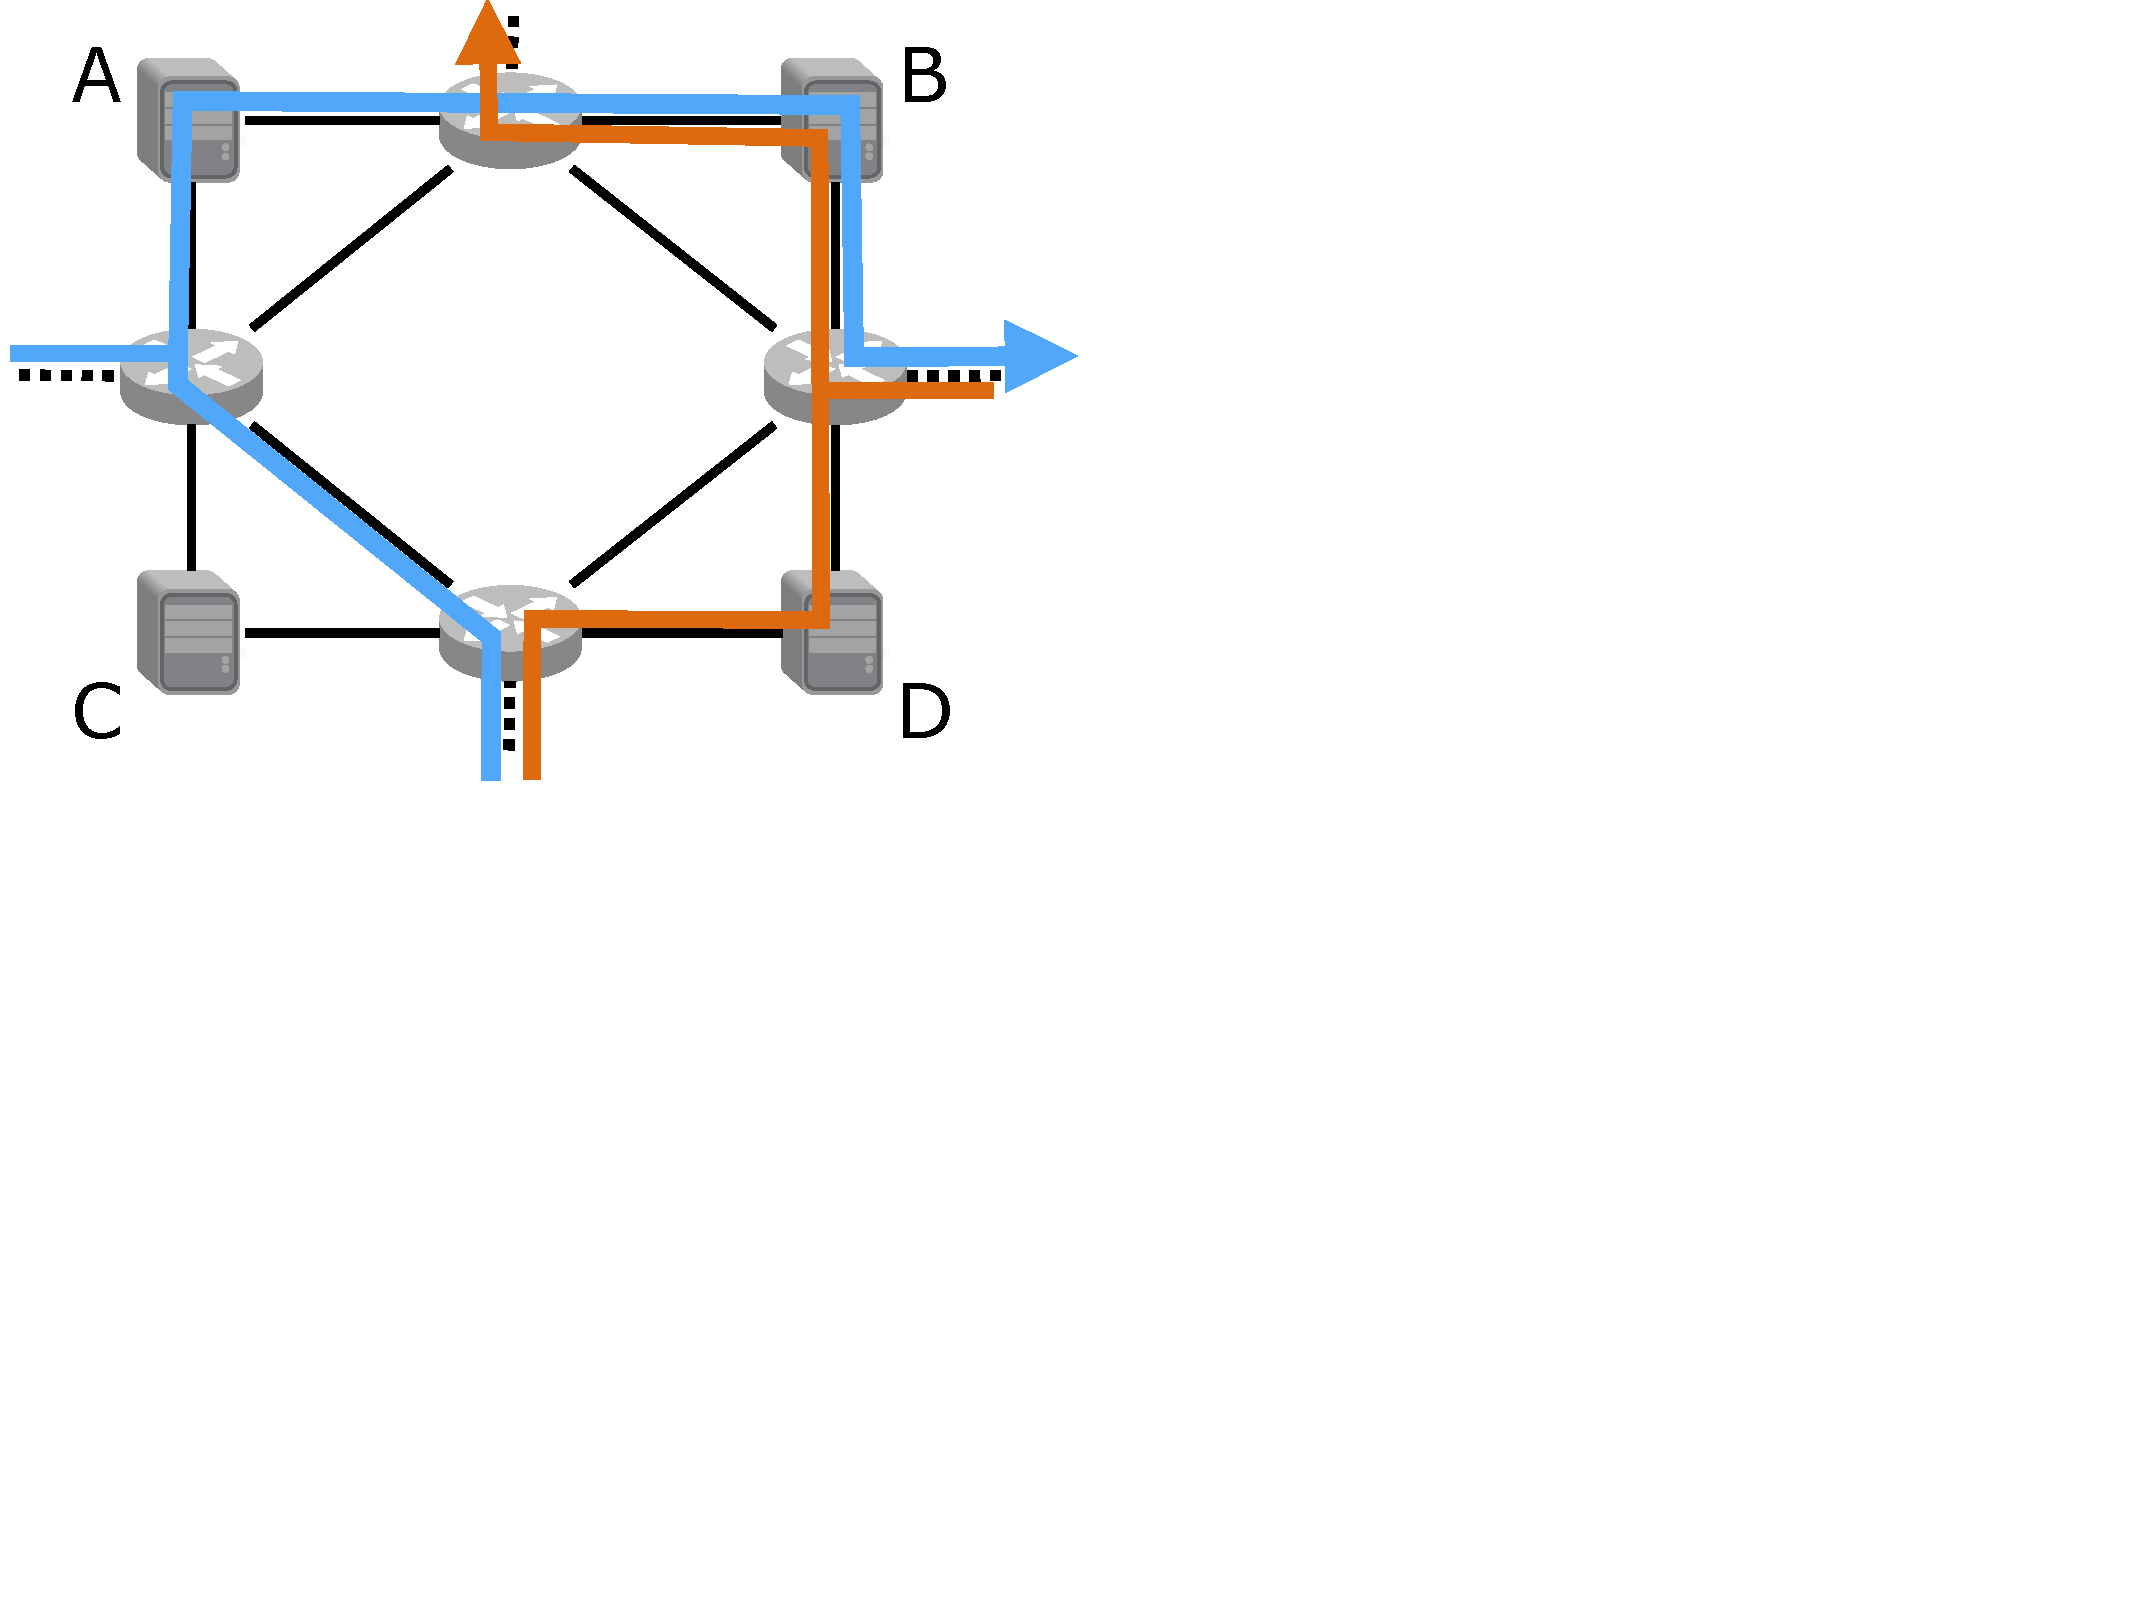
\includegraphics[trim={0 10cm 0 0}, clip, width=\linewidth]{figures/mbox_path_example}
\end{minipage} 
\caption{An illustration of the scaling issues of flat tagging. There are three switches $n_1, n_2, n_3$ and four middleboxes $A,B,C,D$. Packets enter the network on the left and are classified as needing to traverse one of four service chains, and are tagged as such. If flat matching is used, no aggregate rules are possible on the four tags.  }
\label{fig:mbox_path}
\end{figure}
%%%
%%% Matching on sequences
%%%
Fundamentally, the issue is that each AEC is defined by a \emph{collection} of attributes, yet two AECs that differ by only one attribute receive arbitrary, independent indices as tags, preventing switch rules which handle different AECs from being aggregated. For middlebox steering policies, as seen in example figure ~\ref{fig:mbox_path}, AECs are defined by sequences of middleboxes, and two AECs may differ in a single hop.  If tags are assigned such that rules can be aggregated (akin to IP prefix routing), then switches could act upon the packets of multiple AECs with a single rule.
%%%
%%% Capabilities of newer switches 
%%%
Recently, commodity switches have emerged with more sophisticated capabilities, such as OpenFlow 1.3~\cite{of13} switches that supports \emph{wildcard} matching on previously flat header fields, and emerging protocol-independent switches (programmable using languages like P4~\cite{P4}) which support arbitrary headers that can be read, written, and matched in flexible ways.  These advances enable much more flexible ways to tag and match packets, beyond simple index tagging. 

%In the case of virtual circuit switching, the number of possible circuits can be exponential in the size of the network. Switches need to be programmed to react to every tag they may see, resulting in exponential memory usage. It may be the case that the majority of equivalence classes that a switch sees take identical egress ports, yet traditional tagging is unable to take advantage of this redundancy. Fundamentally, an equivalence class can be characterized by a set of attributes where that set is unique to that class. If two circuits differ by only a single hop, their attribute sets are unique and they are assigned different tags. Traditional solutions make no attempt to convey the similarity of the two sets in the tags, which could allow switches to be programmed with a single rule that reacts to both tags. We refer to these solutions as \textit{flat tagging} solutions. 


%Paragraph 3: "In this paper, we show that ...". This is the key paragraph in the intro - you summarize, in one paragraph, what are the main contributions of your paper given the context you have established in paragraphs 1 and 2. What is the general approach taken? Why are the specific results significant? This paragraph must be really really good. If you can't "sell" your work at a high level in a paragraph in the intro, then you are in trouble. As a reader or reviewer, this is the paragraph that I always look for, and read very carefully.

In this paper, we show how the set of attributes that define an equivalence class can be encoded in the assigned tag. The attributes of any tag can then be individually read using a small set of wildcard rules.  Such \emph{attribute-carrying tags} are much more compact, and lead to much smaller rule tables, than index tagging solutions.  We present efficient algorithms for generating compact tags that represent either \emph{sets} or \emph{sequences} of attributes.  We show how these tags can be used to improve the scalability in several real applications, including our SDN-based Internet exchange point~\cite{isdx}.  We have made public the code library for incorporating our tagging scheme into any application. We perform evaluations on both real and synthetic datasets for our proposed applications and show that it can reduce the amount of switch memory by X. 

%Paragraph 4: At a high level what are the differences in what you are doing, and what others have done? Keep this at a high level, you can refer to a future section where specific details and differences will be given. But it is important for the reader to know at a high level, what is new about this work compared to other work in the area.

%Paragraph 5: "The remainder of this paper is structured as follows..." Give the reader a roadmap for the rest of the paper. Avoid redundant phrasing, "In Section 2, In section 3, ... In Section 4, ... " etc.

The remainder of this paper is structured as follows. In \S \ref{sec:background}, we give some area background and a few motivating applications. In \S \ref{sec:flextag_encoding}, we outline the basic ideas of our encoding scheme for attaching sets of attributes to packet headers. In \S \ref{sec:ordering}, we extend our encoding to support ordered sequences of attributes. In \S \ref{sec:identifiers}, we improve the space usage of the encoding. In \S \ref{sec:evaluation}, we evaluate the encoding over both real and synthetic data sets. We discuss related works in \S \ref{sec:related}. The paper concludes with \S \ref{sec:conclusion}.






%\subsection{Common Ground}
%
%Although a diverse set of applications, each of these problems fits a common framework. As a packet enters a local area network, it is classified as belonging to some category of traffic. Associated with this category of traffic is a sequence or set. During classification, this sequence is somehow attached to the packet header.
%All three of these examples have a common framework: Packets are fit into categories as they enter a local area network, and associated with each category is some sequence of information. These sequences can be middleboxes, hosts, next-hop switches, or something else entirely. The sequence could be ordered, as in the case of middlebox paths, or unordered as in the case of feasible next-hops. In each case, the sequence is read by the local network switches to determine which direction to route the traffic. We refer to this reading of information as \textit{membership testing}, because routing choices are decided based upon which hosts or middleboxes are members of the sequence. 

%\subsection{Forwarding Table Matching On Tags}
%
%
%For this scheme of attaching information sets to packets to be feasible with commodity switches, it must be possible for membership testing to be implemented in the forwarding tables of switches. In switch TCAM tables, rules are are comparisons between a fixed string and the packet header, where the fixed strings are over the alphabet $\{0,1,*\}$. $0$ and $1$ are specific bit values, and $*$ denotes "don't care". We say that a packet header matches a string if for every bit in the header, either the bits are equal or one is a wildcard. Example usages include exact matches (strings with no wildcards), prefix matches (strings that end in wildcards), and reading of individual bits (strings with only one non-wildcard). 
%
%Various applications benefit from the use of TCAM 
%
% (TODO: cite some tagging works like flowtags and the original SDX?) have solved the problem of associating packets with information sets by generating a tag for each unique information set and repurposing one of the fields in the header for the tag. In the FlowTags work, each middlebox path had its own set of tags, which could fit into the IP Fragment Identification field. To determine if middlebox $X$ is the next-hop, switches must compare the tag to every tag which has $X$ as a next-hop using TCAM exact matches. This can result in a TCAM entry count exponential in the number of bits in a tag. In the SDX work, each set of next-hops had a unique tag which was placed in the destination mac field. Again, to determine if next-hop $X$ is correct, the tag must be compared against every tag which contains $X$ using exact TCAM matches. 
%
%In both works, the number of bits required can be quite small, but membership tests are expensive, requiring rules exponential in the tag size. TCAM is a very limited resource, and it would be desirable to design tags with the goal of decreasing the number of entries required for membership testing. 
%
%To combat these issues, we present a compression scheme which allows
%the encoding of sequences over a large number of elements, such as service chains or lists of BGP next-hops, into a format easily queried by commodity switches. We show how, with an additional algorithm, this scheme can be used to compress both ordered and unordered sets. Finally, we evaluate our algorithms across both synthetic and real datasets, and show not only does the number of bits needed by our compression scheme compete with the number of bits needed by tags, but that that each core switch need only a constant number of entries per membership test, versus a linear number of entries for the case of flat tagging.


